% !TeX root = ../main.tex
% Add the above to each chapter to make compiling the PDF easier in some editors.

\chapter{Design and Implementation}\label{chapter:design}

The goal of this work is to design a system that will allow the verification of closed peer reviews without a trusted third party. The new artefact should improve the existing ones, which are the current peer review showcase platforms. Based on the problems identified, the requirements of such a system is defined in the following section. Taking these requirements and available technologies into account, a design of system will be communicated. Additionally, the implemented proof of concept prototype will be demonstrated.

\section{Requirements}

As stated in the problem statement, current lack of recognition of peer reviews stems from the public unavailability of the closed peer reviews. Each individual party presented with the peer reviews of a researcher needs to explicitly contact each journal if they want to verify the peer reviews. This is clearly infeasible in a public setting: if a researcher has their peer reviews stated in a public profile, e.g. on their website, each party consuming this data has to contact the journals. This is not the case for other scholarly works such as manuscripts. Therefore, it should be easy to check if the peer review has taken place, that is, the peer reviews are \textbf{verifiable}.

Currently, there are platforms for aggregating and showcasing peer reviews. The process of adding peer reviews to these platforms include automatic methods such as integrations with journals. Users can also add reviews manually such as by sending the review receipt emails or by filling out the review information on the platform. These will get checked by the platform and then the peer review will be "verified". However, it is not possible to trace how the the review is verified and it is at the platforms discretion to decide what constitutes a verified review and what is not. It is possible to see researchers on these platforms that have over 1000 verified reviews per year on their profile. Questions about the validity of this data has been raised \parencite{TeixeiradaSilva.2020, TeixeiradaSilva.2017, TeixeiradaSilva.2019} and it is important to provide provenance on data and \textbf{transparency} on how the verification is done. 

It is difficult to define openness in science. Here we refer to the openness of data. Although there is an inherent conflict with the nature of the closed reviews and the availability of the data, it should be a goal to maximize the openness of data as much as possible. This may include open source.

A peer review has various metadata associated. The necessary data to presented may be different in each context. For a review author it is useful to be able present different data associated with the review without breaking the verifiabilty of the review. For instance, the contents and the date of a closed review may not be shared on a public profile, but a review author might want to share these in a more private setting such as in a job or grant application. In both cases, the reviewer should be able to \textbf{selectively disclose} which attributes they want to share.

A user should be able to take their data and migrate into another platform easily. Avoid vendor lock-in. 

There are many flavors of peer review. Each process may have different data associated. It should be possible to create different attributes for a review without breaking compatibility.

Here the requirements are listed together once again.
\begin{enumerate}
  \item Verifiablity
  \item Transparency
  \item Openness
  \item Selective Disclosure
  \item Portability
  \item Extendability (compatibility)
\end{enumerate}

\section{Design}

\subsection{Overview}

We choose to base our design on W3C's Verifiable Credentials specification \parencite{Sporny.18Kas2019}. The specification inherently satisfies some of the requirements of our systems. It is verifiable..... Also, there exist open source libraries that can be used in implementation.

The designed system has two main components:

\begin{enumerate}
    \item \textbf{Journal X:} A hypothetical journal that issues peer review credentials
    \item \textbf{Veriview:} A peer review showcase platform that supports VCs
\end{enumerate}

In a typical peer review process, a researcher receives an invitation to peer review from the editor of the journal. Here, upon receiving an invitation from Journal X, the author researcher accepts it and submits the review of the manuscript to Journal X. Then she can request the proof of their work as a peer review verifiable credential. Journal X prepares the credential and issues it by signing. The review author can use this credential to prove their authorship. This can be a private exchange with an employer or a colleague. In our system we also conceive a peer review showcase platform called Veriview, where review authors can build their "peer review resume". According to the privacy policy of the review, they can decide which information about the review to share publicly.

An overview of the interactions of the typical use case on the system are depicted below in Figure \ref{fig:sequence1} 

\begin{figure}[htpb]
  \centering
  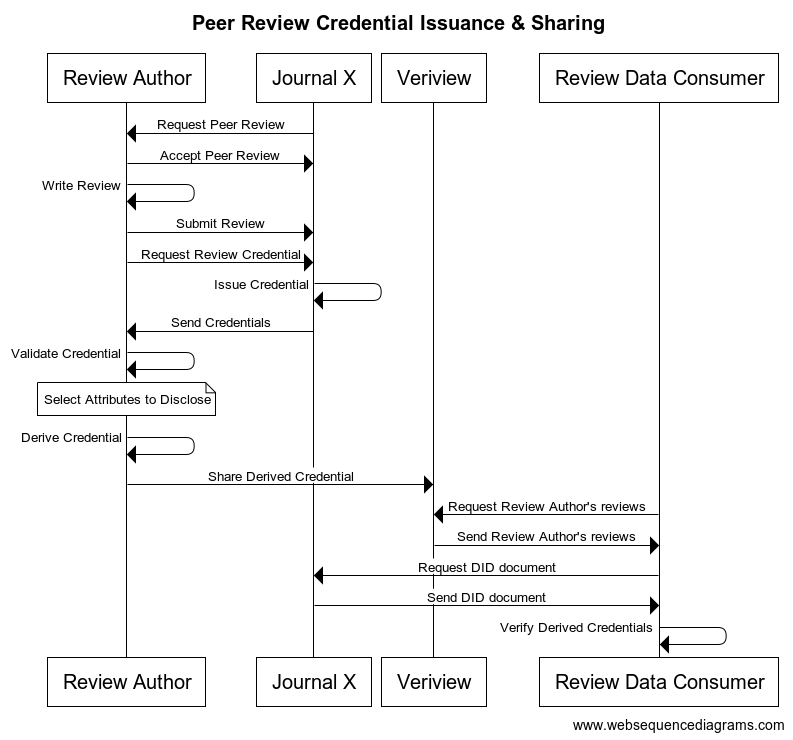
\includegraphics[width=0.8\textwidth]{figures/sequence.png}
  \caption{Overview of peer review issuance and sharing process} \label{fig:sequence1}
\end{figure}

Additionally we assume a "Review Data Consumer", a party which is interested in the peer review data of a reviewer. In real world these might be employers, university, research institutions, or other researchers. Any party that is interested in the peer reviews of a researcher, and their authenticity, might be a consumer. 

The use case depicted in Figure \ref{fig:sequence1} assumes the reviews are shared publicly and are not open reviews. Since Veriview is a platform to share peer reviews publicly, the review author will choose which attributes they want to and are able to share, and derive a credential containing the selected attributes and a zero-knowledge proof which can be shared in Veriview. 

In a private setting or for an open review this additional derivation step is not required. For instance, if the researcher wants to show their review in a grant application, they might want to share the reference to the manuscript and the contents of the review. If the manuscript is in the scientific field the researcher wants to show competence in, being able to verifiably show that they were invited and done a review in this field  would demonstrate the researchers competence. Also, other factors such as the journal's reputation provide additional information. In this case Veriview is not required and the interactions are as in Figure \ref{fig:sequencePrivate}.

\begin{figure}[htpb]
  \centering
  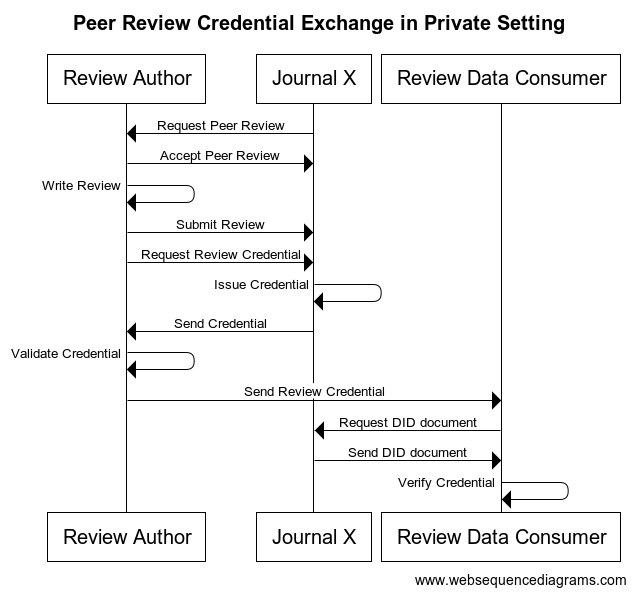
\includegraphics[width=0.8\textwidth]{figures/sequencePrivate.png}
  \caption{Peer Review Credential Exchange in a Private Setting} \label{fig:sequencePrivate}
\end{figure}

\subsection{Peer Review Credential}

The Peer Review Credential is a document issued by a journal that a peer review has been done for this journal. The document contains the review content and the metadata associated such as the date, title, author etc. An example credential is given below in Listing \ref{lst:exampleReview}

\lstinputlisting[language=json, caption={Example Peer Review Credential},label={lst:exampleReview}]{code/exampleReviewCredential.json}

The credential in this design follows the JSON-LD syntax. JSON-LD is the preferred format used as the VC specification and many of the VC libraries available are JSON-LD based. 

\lstinline{@context} defines the vocabularies used in the document. The first URL refers to the VC context and it is required to be included in all verifiable credentials according to the specification. The second context contains the vocabulary for peer reviews. We also provide a vocabulary for our system specific for the peer reviews, but any vocabulary can be used. Thanks to the extensibility of Verifiable Credentials, it possible to extend the vocabulary itself, or include other vocabularies in the document. For instance, if the peer review process of a journal has a statistical soundness check, this can be represented as a \lstinline{statisticallySound} field defined in another vocabulary. Although, it is important these vocabularies are accepted by the ecosystem to maintain the interoperability. Finally, \lstinline{https://w3id.org/security/bbs/v1} provides the vocabulary for the \lstinline{BbsBlsSignature} since it is not included in the default \lstinline{https://www.w3.org/2018/credentials/v1} context.

\subsubsection{Decentralized Identifiers}

Decentralized Identifiers and Verifiable Credentials are both part of the Self-Sovereign Identity ecosystem. Still, both specifications are separate and do not depend on each other. 

Since DIDs are URLs, they can be used in the fields that require to be URLs in VCs. This includes \lstinline{id} fields, \lstinline{issuer}, \lstinline{verificationMethod}. Using DIDs in \lstinline{issuer} and \lstinline{verificationMethod} leverages the public keys associated with DIDs.


\subsection{Peer Review Credential Issuance}


\subsection{Peer Review Credential Verification}


\subsection{Peer Review Credential Derivation}


\subsection{Derived Credential Verification}

\subsection{The Role of Distributed Ledgers}

\subsection{Evaluation of Requirements}















\section{Prototype}

A working proof of concept application is developed to demonstrate the technical feasibility of the proposed solution. The source code is open and available at GitHub \footnote{https://github.com/kuzdogan/peer-review-verifiable-credentials-thesis}. Thanks to the vibrant community around VCs and SSI, and existing open source libraries it was possible create a working prototype. The implementation mainly relies on the jsonld-signatures-bbs library \footnote{https://github.com/mattrglobal/jsonld-signatures-bbs} by MATTR global \footnote{https://mattr.global/} which is a cryptographic suite of BBS+ signatures to sign, verify, and selectively disclose JSON-LD documents. Since VCs adapts JSON-LD as one of its representation formats, the library can be used for VC implementations as well.

To simulate a typical peer review workflow two different applications were developed: a simple journal management system for submitting and reviewing manuscripts, and a peer review aggregation platform that accepts BBS+ peer review VCs. Overall the interactions from a reviewer's perspective is depicted in Figure .
